In this section a range of tests will be conducted on different NPG structures in order to uncover the effect of manipulation of the bridges between the GNR's in NPG. From an applied perspective, one of the main motivations is to find out how these bridges can be manipulated in order to control the current through the material. Some studies has already shown how one could possibly confine the current flow to a single GNR channel by manipulation of bridges between GNR's utilising \textit{Quantum Interference} effects, thus providing a solution to an important aspect in carbon-based nanocircuitry design, namely confinement of electron flow. The study was focused on the difference in effect of having \textit{meta} and \textit{para} bridges between the GNR's. Meta and para bridges are essentially benzene rings oriented in two different ways, see \cref{}. This section will be, in part, an attempt to reproduce some of the results of the study and also to see what happens if other species of atoms are added to these benzene rings in the meta and para bridges. In \cref{} the difference between the structures can be seen in relation to the bridges of the normal NPG. The bridges will be manipulated by insertion of either Oxygen atoms or Hydroxide molecules. The atoms/molecules will be inserted on each side of a GNR either in a symmetric or asymmetric fashion (see \cref{}). In \cref{testtable} a schematic overview of the different systems, subject to tests, can be seen. 
\begin{table}[ht]
\begin{tabular}{cclcll}
		\toprule
		Test no. & Meta/Para & Symmetry   & No. of species & Added species & Name  \\ \midrule
		1        & Para      & Symmetric  & 4              & Oxygen        & PS4O  \\
		2        & Para      & Symmetric  & 4              & Hydroxide     & PS4OH \\
		3        & Meta      & Symmetric  & 2              & Oxygen        & MS2O  \\
		4        & Meta      & Symmetric  & 2              & Hydroxide     & MS2OH \\
		5        & Meta      & Asymmetric & 2              & Oxygen        & MA2O  \\
		6        & Meta      & Asymmetric & 2              & Hydroxide     & MA2OH \\
		\bottomrule
	\end{tabular}
	\caption{Table showing an overview of all the structures that will be tested in this section.  How the different species will be manipulated during the tests, will be stated in plots produced for results. The code names follow the table column-wise. In \cref{appfigs}, \cref{Strucow} a collection of figures showing each scenario stated in this table.}
\label{testtable}
\end{table}
The results from these tests will be presented in the form of band structure plots and they will be compared to band plots produced with DFT and TBtrans. Additionally a schematic overview of the different systems, showing the on-site potentials of each atom will be presented in the figures as well. Following is a section introducing meta and para NPG in detail. 
\subsection{Differences in para and meta bridges}
In broad terms the difference in the meta and para structures lies in the path an electron will travel through the benzene ring to get across the bridge. In the para bridge, the path across the aromatic ring is symmetric and so the electron will pass above or below with equal probability. Since the para bridge has three bonds in each direction across the ring, the path length in the para bridge is the same on each side (See \cref{}). This will cause constructive interference of the states once the waves meet on the other side of the ring, which results in spreading in the density of states from one GNR to the next. For the meta bridge the way across the aromatic ring is not symmetric in the sense that there is two bonds across the path below and four bonds across on the path above (see \cref{}). This will cause a shift by half a wavelength between the two paths and thus create destructive interference between waves meeting on the other side of the ring. The effect of this is confinement in the density of states in the GNR's. In \cref{appfigs},\cref{} 
\subsection{Tests}
In the following sections various tests on the different systems will be conducted using the developed program. The motivation for these test is proposal that NPG can be "tuned" by addition or removal of hydrogen. Tuning with hydrogen is practically feasible, so by using the developed program, it will be possible to simulate different scenarios which will uncover what is going on, chemically as well as physically, in the different NPG system when manipulated. The tests consist of three kind of manipulations. Firstly it will be manipulation of the on-site value for the added oxygen atoms (Addition of Oxygen will be simulated by addition of another carbon site to the structure, effectively adding another pi-electron). Secondly it will be by removal of Hydroxide sites and thirdly by manipulation of the on-site values of Hydroxide. These manipulations may be carried out separately. \\
\subsection{Test 1}
The first test will be manipulation of the system 'PS4O'. The basis structure is para-NPG where 4 carbon sites have been added, two on each benzene ring. Here the carbon atoms added, will be manipulated by lowering their on-site potential of the sites by a value relative to that given by a energy scale from a DFT calculation. This is to simulate adding oxygen. In \cref{PS4O} an overview of the structure can be seen along with the band structure for the system, obtained through DFT and TBtrans. 
\begin{figure}[h]
    \hspace{-2cm}
    \centering
    \begin{subfigure}[b]{0.5\textwidth}
    \centering
    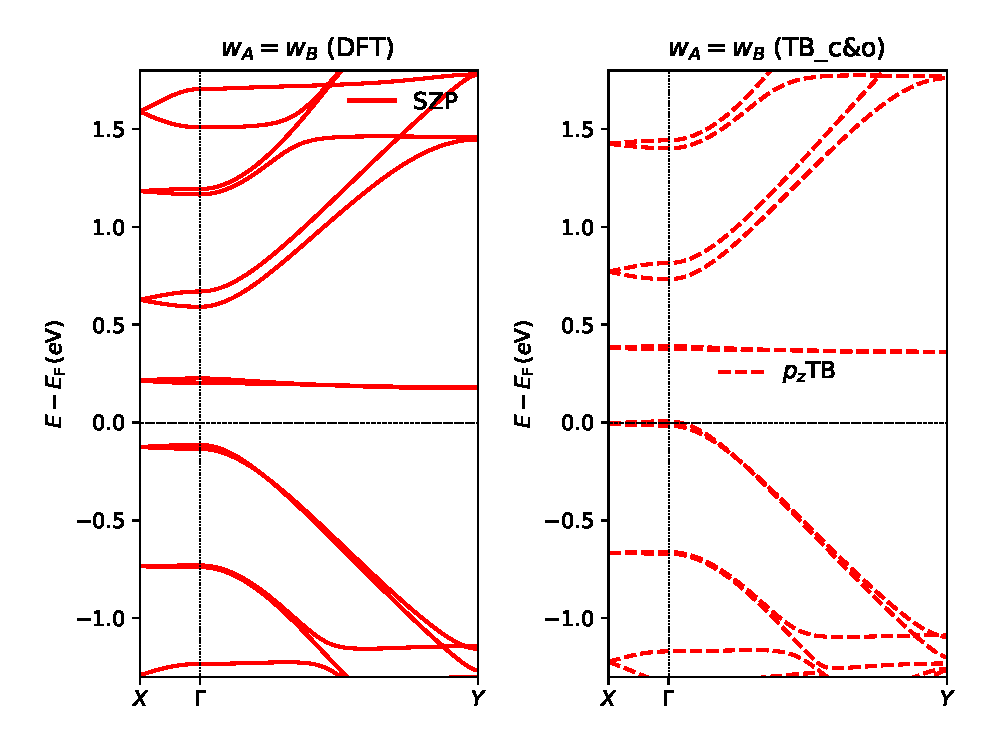
\includegraphics[width=\textwidth]{Figures/p_O4.eps}
    \end{subfigure}
    \vskip\baselineskip
    \begin{subfigure}[b]{0.7\textwidth}
    \centering
    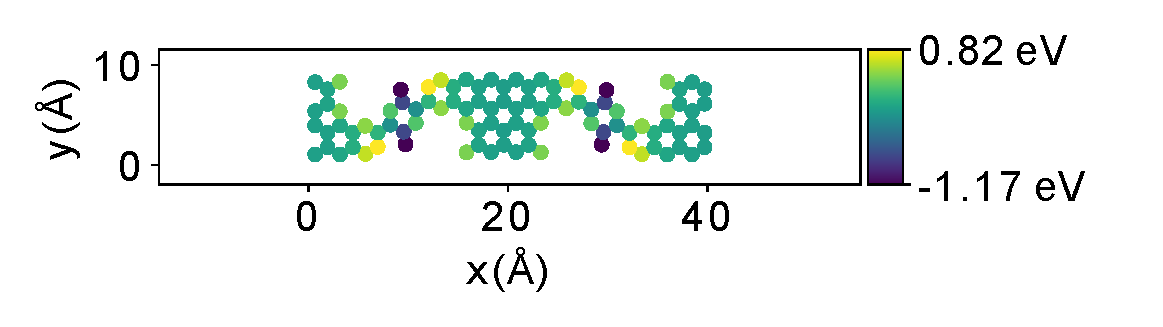
\includegraphics[width=\textwidth]{Figures/PS4O.eps}
    \end{subfigure}
    \caption{Figure showing the band structures obtained using DFT/TBtrans (above) and a potential map of the system (below)}
    \label{PS4O}
\end{figure}
Following, in \cref{PS4Odev} band plots obtained with the developed program is shown. Firstly a band plot without any changes to the on-site potential and next a band plot where the on-site potential of the added sites have been change by an amount corresponding to the lowest value 
\begin{figure}[h]
    \centering
    \begin{subfigure}[b]{0.45\textwidth}
    \centering
    \includegraphics[width=\textwidth]{Figures/}
    \caption{Figure showing the band structures obtained using DFT/TBtrans (above) and a potential map of the system (below)}
    \end{subfigure}
    ~
    \begin{subfigure}[b]{0.45\textwidth}
    \centering
    \includegraphics[width=\textwidth]{Figures/}
    \caption{Figure showing the band structures obtained using DFT/TBtrans (above) and a potential map of the system (below)}
    \end{subfigure}
    \label{PS4Odev}
\end{figure}

The results show that the first plot where no manipulation was done, has some qualitative agreement with the DFT/TBtrans plots. There is two bands at the Fermi level on top of each other showing quantum interference \textit{Where in the structures does these band belong?}. Furthermore  one can see spreading in the first two sets of valence/conduction bands \textit{Again unsure what this corresponds to in relation to the structure}. Note however that the band structure is symmetric around the Fermi level since..\textit{why? Maybe something with the whole thing actually being carbon atoms}. Now if the on-site potential for the added oxygen atom is changed to \(\SI{-0.2}{\electronvolt}\), the band structure changes to something very similar to the DFT/TBtrans plots. There is spreading of the bands at the Fermi level suggesting \textit{what?} and the spreading of the first two pair of valence/conduction bands are also larger. Notice that the Fermi level has had a shift downwards. This may be because of... 
\subsection{Test 2}
Next test will be with the 'xxxx' system. Here the test will show the difference between removing a OH site entirely (effectively the hydrogen in hydroxide removes the extra pi-electron in oxygen from the system, which can be simulated by removing the atoms entirely) and lowering the on-site potential of the oxygen in the OH group significantly in relation to the rest of the system, again by using the energy scale given by the DFT overview. In \cref{somehydroxidefigure} the results of the test is shown. Multiple on-site potentials were tested to see which one came closest to that of the band structures given by DFT/TBtrans. It was found that using values closest to that given by the DFT calculation (\(\SI{xx}{\electronvolt}\)) yielded the best results. Again showing band structures qualitatively close to those obtained from DFT/TBtrans. One can see 
\subsection{Test 3}
\subsection{Test 4}
\subsection{Test 5}
\subsection{Test 6}

%\subsection{Tests with insertion of flour atoms}
%Tests by insertion of flour atoms will be done for both para and meta bridges. Each  of those will be tested with symmetric and asymmetric placement of flour atoms. The configuration of electrons in flour is as such the it does not contribute with any extra pi-electrons to the system and thus adding an extra flour atom to the bridge will still result in an electrostatic system (before injection of an electron). One of the goals of the test is to see whether the effect of adding a flour atom will be global (in relation to the NPG-system) or more localised. Another is to see whether the on-site Hamiltonian along with its hopping matrices will change by addition of a flour atom. 
%\subsection{Tests with insertion of oxygen atoms}
 %Oxygen atoms will be added to the bridges for the first test. The notable difference being that oxygen will add an extra pi-electron to the system. This means that one has to consider the electrostatic effects as well as additional effects from the added pi-electron. Practically, and as an initial test, this is done by adding an extra carbon atoms as a "dummies" for the oxygen atom. Following that one might have to change specific on-site values (the place where the atom is inserted as well as surrounding atoms) to simulate the addition of the oxygen atom. The goal here is to check difference between just adding an extra oxygen (carbon) atom and changing the on-site value.  
%\subsection{Tests with insertion of OH-groups}
%The test case will be insertion of OH-groups. Since the hydrogen atom in the OH-group will remove the extra pi-electron from the equation, one would expect something similar to an electrostatic case. Here there will be a comparison with the normal NPG-para structure...To get results for these tests, the band plot script is used. Simply inputting the structure provided to produce the plots. The Added below each band plot a schematic overview of the systems structure along with on-site potential values calculated from DTF is shown. 
%\subsection{Tests with oxygen/hydroxide mix}
%To test the effects of having one oxygen and one hydroxide group on each bridge. 
